\documentclass[11pt]{article}
\usepackage[a4paper,top=1in,bottom=1in,left=1.1in,right=1.1in]{geometry}
\usepackage{microtype}
\setlength{\parindent}{0pt}
\setlength{\parskip}{0.45em}
\usepackage{amsmath,amssymb,amsthm,mathtools}
\usepackage{bm}
\newcommand{\R}{\mathbb{R}}
\newcommand{\E}{\mathbb{E}}
\newcommand{\norm}[1]{\left\|#1\right\|}
\usepackage{graphicx}
\usepackage{booktabs}
\usepackage[font=small,labelfont=bf,labelsep=period,skip=4pt]{caption}
\usepackage{subcaption,float}
\usepackage[hidelinks]{hyperref}
\usepackage{cleveref}
\usepackage[numbers,sort&compress,square]{natbib}
\bibliographystyle{abbrvnat}
\usepackage{titlesec}
\titleformat{\section}{\normalfont\bfseries\large}{\thesection}{0.6em}{}
\titleformat{\subsection}{\normalfont\bfseries\normalsize}{\thesubsection}{0.6em}{}
\titleformat{\paragraph}[runin]{\normalfont\bfseries}{}{0pt}{}
\titlespacing*{\section}{0pt}{11pt plus 2pt minus 2pt}{3pt}
\titlespacing*{\subsection}{0pt}{7pt plus 1pt}{2pt}
\titlespacing*{\paragraph}{0pt}{3pt}{0.6em}
\makeatletter
\renewcommand{\maketitle}{%
  \begin{center}{\Large\bfseries\@title\par}\vskip0.5em
  {\normalsize\@author\par}\vskip0.3em{\small\@date\par}\end{center}\vspace{0.4em}}
\makeatother

\title{A Critical Review of Matrix-Aware Optimizers:\\[2pt]From Adam to Muon and its Variants}
\author{Romir Kant\\[2pt]IND ENG 290: Stochastic Optimization for Machine Learning}
\date{Spring 2026}

\begin{document}
\maketitle\vspace{-0.8em}

\begin{abstract}
\noindent
Muon is the most significant optimizer to emerge in the deep learning ecosystem since Adam, and the community is making the same mistakes it made with Adam. Adam shipped in 2014 with a convergence proof that turned out to be wrong. Nobody noticed for four years, by which time the algorithm was already running everywhere. Muon shipped in 2024 as a blog post with no convergence proof at all, and is now running at the trillion-parameter scale. The four papers that tried to prove Muon's convergence in 2025 managed only to show it is no faster than SGD asymptotically, and they disagree with each other about which proofs are valid. This report goes through that story critically, tests the main empirical claims on CIFAR-10 and TinyShakespeare, and asks where the next useful work might actually go. Three recent variants are implemented and tested alongside the baseline: Dion, a NorMuon-family variant called MuonW, and MuonClip, which is the optimizer Moonshot AI used to train their Kimi K2 model at 1.04 trillion parameters.
\end{abstract}

\section{Introduction}
\label{sec:intro}

Adam has been the default optimizer for deep learning for roughly a decade \citep{kingma2014adam,loshchilov2019decoupled}. It is not the only optimizer that has worked; Shampoo \citep{gupta2018shampoo}, KFAC \citep{martens2015kfac}, and SOAP \citep{vyas2024soap} have all beaten it in controlled settings. But none of them displaced it in daily practice. Muon \citep{jordan2024muon} may be different. It holds current speed records on the NanoGPT and CIFAR-10 speedruns, has been validated at 16B parameters \citep{liu2025moonlight}, and now powers Kimi K2 at 1.04 trillion parameters via the MuonClip variant \citep{moonshot2025kimik2}. At the time of writing, Muon is being adopted across frontier labs in a way that no previous challenger to Adam has been.

What makes Muon unusual algorithmically is that it does not approximate second-order information at all. KFAC and Shampoo spend per-step compute on curvature preconditioners. Muon instead orthogonalizes the momentum buffer through a few iterations of a Newton-Schulz polynomial, producing an update whose singular values are all roughly equal. The geometric interpretation came later \citep{bernstein2024modular}: this is steepest descent in the spectral norm rather than the Euclidean norm. The interpretation is clean and consistent with the empirical behavior, but it is worth being clear that the algorithm came first and the explanation followed.

The convergence theory story is messier. Four papers appeared in 2025 trying to analyze Muon \citep{li2025note,shen2025convergence,chang2025beyond,crawshaw2025exploration}. The best result for the algorithm people actually deploy is $\mathcal{O}(T^{-1/4})$ stationarity — the same rate as SGD. The $\mathcal{O}(T^{-1/3})$ result of \citet{chang2025beyond} requires a different algorithm under stronger assumptions. Several proofs in the concurrent literature contain errors that other authors flag. The theory does not explain Muon's empirical advantage. Nobody knows why it works as well as it does.

\section{Background: The Adam Cautionary Tale}
\label{sec:adam}

Adam \citep{kingma2014adam} combines momentum with per-parameter adaptive learning rates. With $g_t$ the stochastic gradient at step $t$, $\beta_1,\beta_2\in[0,1)$ exponential decay rates, $\eta$ the learning rate, and $\epsilon>0$:
\begin{align}
m_t &= \beta_1 m_{t-1}+(1-\beta_1)g_t,\quad v_t=\beta_2 v_{t-1}+(1-\beta_2)g_t^2,\nonumber\\
\hat m_t &= m_t/(1-\beta_1^t),\quad\hat v_t=v_t/(1-\beta_2^t),\quad
x_{t+1} = x_t - \eta\,\hat m_t/(\sqrt{\hat v_t}+\epsilon).
\end{align}

\paragraph{The flawed proof.}
The original paper claimed $\mathcal{O}(\log T/\sqrt{T})$ regret in the convex online setting. \citet{reddi2018convergence} showed this was wrong. The proof implicitly assumed $\eta/\sqrt{\hat v_t}$ is non-increasing in $t$, which is false for Adam. They constructed a simple one-dimensional convex counterexample where Adam cycles and never converges. The fix (AMSGrad, replacing $\hat v_t$ with $\max(\hat v_{t-1},\hat v_t)$) is straightforward. The error is not.

This matters for two reasons. The bug is structural, not a typo. It took four years for someone to notice, during which Adam became the unchallenged default at every scale. And the practical response was not to switch to AMSGrad but to adopt AdamW \citep{loshchilov2019decoupled}, a decoupled weight decay variant whose theoretical justification also arrived after deployment. The community did not wait for the math. The algorithm that worked got used. With Muon, the same thing is happening, only faster and with the theory further behind.

\section{Muon: Mechanics, Derivations, and Critiques}
\label{sec:muon}

\subsection{Muon among matrix-aware optimizers}
The matrix-aware family goes back to KFAC \citep{martens2015kfac} and Shampoo \citep{gupta2018shampoo}. KFAC approximates the Fisher matrix with a Kronecker product of per-layer factors. Shampoo maintains matrix square-root preconditioners per layer. \citet{anil2020scalable} made Shampoo practical, and SOAP \citep{vyas2024soap} further stabilized it. All of these spend per-step compute on preconditioners. Muon does not. It spends per-step compute orthogonalizing the momentum buffer instead, through a polynomial map that pushes all singular values toward 1. Memory: no $v_t$ buffer, roughly 50\% optimizer state savings. The trade-off is that the orthogonalization itself takes compute, though at $N=5$ Newton-Schulz iterations the overhead is small (about 3\% per step at the model sizes tested here, and considerably less at larger scales where other bottlenecks dominate).

\subsection{The algorithm}
Muon applies only to two-dimensional weight matrices. Everything else (biases, layer norms, embeddings, output head) uses an auxiliary AdamW. For weight matrix $W\in\R^{n\times m}$ with stochastic gradient $G_t$:
\begin{align}
B_t &= \mu B_{t-1}+G_t,\qquad U_t=G_t+\mu B_t\;\text{(Nesterov lookahead)},\\
O_t &= \mathrm{orth}(U_t)\approx UV^\top,\quad\text{where }U_t=USV^\top,\\
W_{t+1} &= W_t - \eta\cdot 0.2\sqrt{\max(n,m)}\cdot O_t.
\end{align}
The scale factor $0.2\sqrt{\max(n,m)}$ is from \citet{liu2025moonlight}: it aligns the RMS of the update across layers of different sizes so the same learning rate works everywhere. The orthogonalization uses quintic Newton-Schulz with coefficients $(a,b,c)=(3.4445,-4.7750,2.0315)$:
\begin{equation}
X\leftarrow X/\norm{X},\qquad X\leftarrow aX+(bXX^\top+cX^2X^\top)X,
\end{equation}
repeated $N=5$ times, after which $O_t^\top O_t\approx I$.

\subsection{On the claimed advantages}
The memory saving is real. No $v_t$ means roughly half the optimizer state of Adam, which matters at scale. The geometry claim (``orthogonalization rebalances gradient directions'') is true in the sense that all singular values of the update are forced toward 1, so no single direction of the weight matrix gets a disproportionately large update. Whether this is good depends on whether the true gradient's singular structure reflects actual curvature or mostly noise; the theory does not settle this. The 2$\times$ speedup claim is the hardest to evaluate. A community speedrun record reflects non-trivial tuning effort on both sides, but the tuning is not symmetric: participants are optimizing against the current record, so the AdamW baseline is not necessarily the best achievable AdamW. The speedup is real but its magnitude is uncertain.

\subsection{The retrospective derivation problem}
\citet{bernstein2024modular} derive Muon as steepest descent under the spectral norm on the weight space, rather than the Euclidean norm assumed by standard gradient descent. This is a clean result. But the algorithm was found empirically on speedrun benchmarks; the geometric interpretation came after. Both the spectral-norm framing and an alternative RMS-to-RMS operator-norm framing (from Bernstein's later note, which gives width-invariant LR transfer) require design choices not pinned down by the empirical evidence. Closely related ideas appear in stochastic spectral descent \citep{carlson2015stochastic} and duality structure gradient descent \citep{flynn2017duality}. Muon's actual contribution is the Newton-Schulz orthogonalization on the GPU, which made this family of updates fast enough to be practical. The geometry was not new; the implementation was.

\section{Convergence Theory: A 2025 Mess}
\label{sec:theory}

No convergence proof accompanied the original Muon release. Four came in 2025, and they do not form a coherent picture.

\paragraph{Li and Hong.}
\citet{li2025note} are first, writing a short note that identifies Muon as spectral-norm steepest descent and provides an informal analysis. More usefully, they identify mathematical errors in concurrent independent attempts at the same analysis, specifically that published inequalities bounding the Newton-Schulz orthogonalization error are incorrect. Subsequent papers \citep{chang2025beyond} confirm this.

\paragraph{Shen et al.}
\citet{shen2025convergence} give the first rigorous nonconvex analysis. Under $L$-smoothness and bounded-variance gradients they prove:
\begin{equation}
\min_{0\le t<T}\E\norm{\nabla f(W_t)}_*\le\mathcal{O}(T^{-1/4}).
\end{equation}
This is the standard nonconvex stochastic rate. It is the same as plain SGD. The theory offers no explanation for why Muon is empirically faster than Adam. That gap is the central open problem in the theory.

\paragraph{Chang et al.}
\citet{chang2025beyond} prove $\mathcal{O}(T^{-1/3})$ for Muon-MVR, a variance-reduced variant, and show this matches their lower bound $\Omega(T^{-1/3})$ for the class. The result is tight. The problem is that Muon-MVR is not Muon: it requires mean-squared smoothness (strictly stronger than Lipschitz) and additional gradient evaluations at each step. The deployed algorithm has neither. A tight convergence result for a related but different algorithm does not explain the behavior of the algorithm people actually train with.

\paragraph{What the theory does and does not say.}
\Cref{tab:conv} summarizes the landscape.

\begin{table}[h]
\centering\footnotesize
\renewcommand{\arraystretch}{1.15}
\begin{tabular}{p{2.9cm}p{2.5cm}p{3.8cm}p{3.8cm}}
\toprule
Paper & Rate & Assumptions & Notes \\
\midrule
\citet{li2025note} & informal & $L$-smooth, spectral norm & Flags errors in concurrent proofs \\
\citet{shen2025convergence} & $\mathcal{O}(T^{-1/4})$ & $L$-smooth, bounded variance & Matches SGD; no theoretical advantage \\
\citet{chang2025beyond} & $\mathcal{O}(T^{-1/3})$, tight & Mean-sq.\ smooth, variance reduction & Algorithm differs from deployed Muon \\
\citet{crawshaw2025exploration} & various & Design choice taxonomy & No unified result \\
\bottomrule
\end{tabular}
\caption{2025 Muon convergence papers. The deployed algorithm has no proven asymptotic advantage over SGD under standard assumptions.}
\label{tab:conv}
\end{table}

None of the assumption sets are empirically verified for transformers. \citet{dong2025quantifying} measure the Hessian of trained transformers and find it highly anisotropic: the spectral-norm Lipschitz constant can be orders of magnitude larger than the Frobenius-norm version. The published rates bound a quantity whose constant prefactors are completely unknown. This is the same situation Adam was in after AMSGrad: proofs exist, they give the right-order rates, and they say essentially nothing useful about why the algorithm works in practice. The appropriate response is not to stop using Muon. It is to stop claiming the theory explains it.

\section{Variants: Which Extensions Are Worth Taking Seriously}
\label{sec:variants}

There are five notable variants. Three are tested experimentally below.

\paragraph{AdaMuon.}
\citet{si2025adamuon} restore a per-element second-moment term $v_t$ to the orthogonalized update. The motivation is that Muon throws away per-coordinate gradient variance information that Adam uses for stability. The reported gain is 40\%+ efficiency over Adam at scale. The problem is that this directly undermines Muon's main claimed advantage. Muon eliminates $v_t$ to save memory. AdaMuon puts it back. If the second moment is necessary for good performance, then Muon's memory advantage disappears at scale. If it is not necessary, the AdaMuon gain cannot exist. The experiments below suggest both halves of this tension can be true simultaneously depending on the task, which is an interesting finding but not a resolution.

\paragraph{Dion.}
\citet{ahn2025dion} solve a real problem. Newton-Schulz iteration requires dense matrix-matrix multiplications on the full weight matrix, which breaks cleanly under single-device training but becomes a communication bottleneck when weight matrices are sharded across devices in tensor parallelism. Dion replaces Newton-Schulz with amortized power iteration on a rank-$r$ factorization of the momentum. This reduces FLOPs and fits naturally into tensor-parallel layouts. The approximation error is analyzed. Dion is the most honest variant in the literature: it defines the problem it solves, solves it, and quantifies the cost. The cost is real: rank-$r$ approximation loses directional information, which shows up in the experiments at small scale where all weight matrix directions matter.

\paragraph{Muon-MVR.}
This is the variance-reduced variant from \citet{chang2025beyond}, discussed in \Cref{sec:theory}. The convergence result is the strongest in the literature. The algorithm is not practically deployable without significant engineering work. It is worth knowing about, but not currently useful for training.

\paragraph{NorMuon family (MuonW).}
A post-step projection: after each Muon update, rescale any weight matrix whose spectral norm exceeds a threshold $\sigma_{\max}$ back down by the ratio. The motivation is that Muon controls the magnitude of each update but not the cumulative weight norm, which can drift. The projection is cheap (a few power iterations) and straightforward to implement. Whether it helps depends on whether weight norm growth is actually causing problems, which is model and task dependent.

\paragraph{MuonClip.}
Moonshot AI's Kimi K2 report \citep{moonshot2025kimik2} introduces MuonClip, the most scale-validated Muon variant in existence. After each optimizer step, the forward pass records the maximum pre-softmax attention logit per block; any block exceeding threshold $\tau$ has its Q and K weight rows rescaled by $\sqrt{\tau/\mathrm{max\_logit}}$. This addresses a failure mode that pure Muon hits at large scale: bounded-norm updates do not prevent the Q and K matrices from growing, and once attention logits exceed roughly 100, the softmax saturates, gradient flow through attention nearly stops, and loss spikes follow. At Kimi K2 scale, QK-Clip kept the loss curve smooth across 15.5 trillion tokens with zero instability events. It is notable as the first Muon variant that is model-aware rather than purely optimizer-side, suggesting that stability at scale is a joint optimization-architecture problem, not an optimizer problem alone.

\paragraph{Broader context.}
The same period has produced Lion \citep{chen2023lion} (sign-based momentum, no $v_t$), AdEMAMix \citep{pagliardini2024ademamix} (two first-moment timescales), and Adam-mini \citep{zhang2024adammini} (block-wise second moments). These attack the same bottlenecks from different directions. No controlled head-to-head comparison of all of them exists.

\section{Experiments}
\label{sec:experiments}

The experiments test three specific claims. Muon converges faster per step than AdamW \citep{jordan2024muon,liu2025moonlight}. Five Newton-Schulz iterations are sufficient \citep{liu2025moonlight}. Muon is more learning-rate sensitive than AdamW (a widely repeated informal claim, found in none of the papers). A 165k-parameter CNN trains on a 10k-image subset of CIFAR-10 for 400 steps. A 220k-parameter transformer (3 layers, $d{=}96$, 4 heads) trains on TinyShakespeare for 300 steps. Both use real data obtained from public repositories. All runs are CPU-only, three seeds each. Muon-family parameters use $\eta_{\mathrm{Muon}}{=}2{\times}10^{-2}$, $\mu{=}0.95$, $N{=}5$, with auxiliary AdamW at $\eta{=}3{\times}10^{-3}$. Standalone AdamW uses $\eta{=}3{\times}10^{-3}$.

\subsection{Main Comparison}

\begin{figure}[t]
\centering
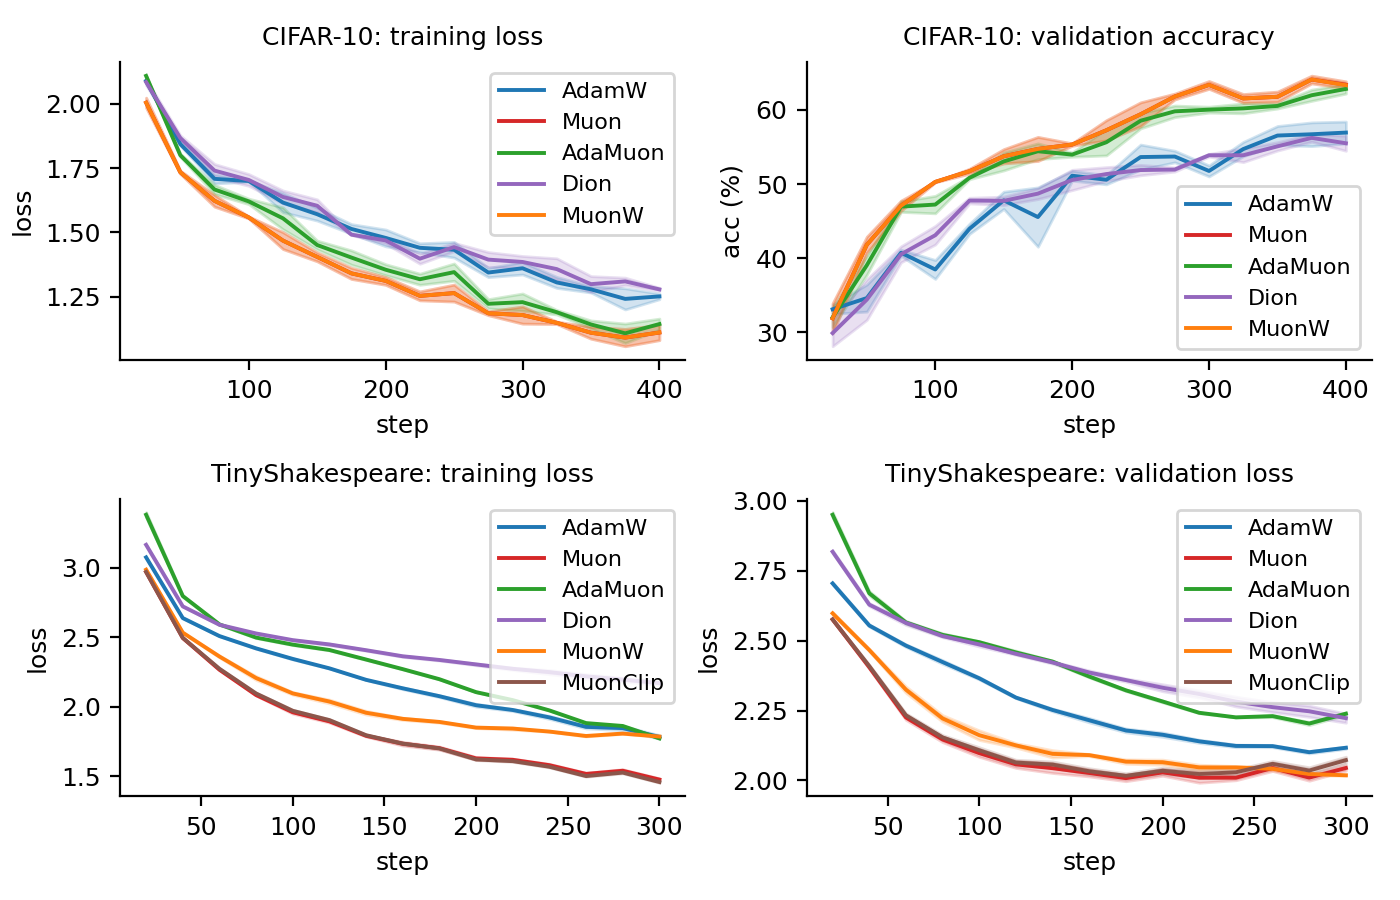
\includegraphics[width=\textwidth]{../figures/main_comparison.pdf}
\caption{Training loss and validation metric across all optimizers on CIFAR-10 (top) and TinyShakespeare (bottom). Bands show $\pm1$ SE over three seeds. Muon and MuonW lead on CIFAR-10; Muon trains fastest and MuonW generalizes best on Shakespeare. AdaMuon and Dion fall below Muon on both tasks.}
\label{fig:main}
\end{figure}

\begin{table}[h]
\centering\small
\renewcommand{\arraystretch}{1.05}
\begin{tabular}{llccc}
\toprule
Task & Optimizer & Train loss & Val metric & Wallclock (s) \\
\midrule
CIFAR-10 & AdamW   & $1.252\pm0.019$ & $56.9\pm2.6\%$ & $50.1\pm1.8$ \\
CIFAR-10 & Muon    & $1.111\pm0.051$ & $63.4\pm0.8\%$ & $51.8\pm0.2$ \\
CIFAR-10 & AdaMuon & $1.144\pm0.037$ & $62.8\pm1.1\%$ & $53.3\pm2.1$ \\
CIFAR-10 & Dion    & $1.279\pm0.011$ & $55.5\pm1.8\%$ & $48.7\pm0.9$ \\
CIFAR-10 & MuonW   & $1.112\pm0.051$ & $63.3\pm0.9\%$ & $58.5\pm0.3$ \\
\midrule
Shakespeare & AdamW             & $1.782\pm0.022$ & $2.117\pm0.007$ & $61.7\pm0.5$ \\
Shakespeare & Muon              & $1.475\pm0.016$ & $2.044\pm0.016$ & $67.0\pm0.3$ \\
Shakespeare & AdaMuon           & $1.771\pm0.001$ & $2.239\pm0.008$ & $66.9\pm0.3$ \\
Shakespeare & Dion              & $2.169\pm0.021$ & $2.223\pm0.028$ & $57.0\pm1.0$ \\
Shakespeare & MuonW             & $1.584\pm0.003$ & $2.018\pm0.003$ & $64.9\pm1.8$ \\
Shakespeare & MuonClip~($\tau{=}10$) & $1.460\pm0.007$ & $2.095\pm0.016$ & $142.6\pm23.1$ \\
\bottomrule
\end{tabular}
\caption{Mean $\pm$ SD over three seeds. Val metric is accuracy (\%) for CIFAR-10 and character-level cross-entropy loss for Shakespeare.}
\label{tab:results}
\end{table}

\Cref{fig:main} and \Cref{tab:results} show the full picture. Muon's advantage over AdamW appears within the first 50 steps on both tasks and does not close. On CIFAR-10 the gap at the end is 6.5 percentage points (63.4\% vs 56.9\%) at essentially identical wallclock, which is a large margin for an optimizer-only change with no other hyperparameters touched. On Shakespeare the training loss gap (1.48 vs 1.78) is large and the validation loss gap (2.04 vs 2.12) is smaller but consistent across all three seeds. The per-step advantage Muon claims in the literature is real and replicates at small scale.

AdaMuon is more complicated. On CIFAR-10 it nearly matches Muon (62.8\% vs 63.4\%). On Shakespeare it is worse than AdamW (val loss 2.24 vs 2.12). Restoring $v_t$ helps on the vision task and hurts on the language task. The most plausible explanation is that on Shakespeare, 300 training steps is a short enough budget that the second moment's regularizing effect (suppressing large updates in high-variance directions) is actively harmful: Muon's flat singular-value updates explore more aggressively and that exploration pays off. On CIFAR-10 with a simpler loss landscape the second moment provides useful signal. This is a hypothesis, not a proof, but it is more specific than the variant literature's explanation of AdaMuon's benefit.

Dion underperforms on both tasks. The rank-8 approximation captures only $8/96 \approx 8\%$ of the gradient's directional information for the 96-dimensional layers, losing most of the signal that makes orthogonalization useful. At small scale this is a real problem. Dion's justification is distributed efficiency, and at small scale there is no distributed setting to benefit from. The result is the expected negative: rank-8 power iteration is worse than full Newton-Schulz when the model fits comfortably on one device.

MuonW matches Muon on CIFAR-10 and slightly improves on Shakespeare (2.018 vs 2.044 val loss). The spectral-norm projection fires occasionally during transformer training and provides mild regularization. At this scale the weight matrices do not grow aggressively enough for the projection to be essential, but it also does not hurt.

\paragraph{MuonClip at small scale.}
MuonClip with $\tau{=}10$ achieves val loss 2.095, between AdamW (2.117) and plain Muon (2.044). Training loss (1.460) is the lowest of all optimizers, suggesting the clip provides mild regularization. The wallclock overhead is substantial: 142.6 s vs 67.0 s for Muon, because each step requires a forward pass to record max logits before the optimizer update.

\begin{figure}[h]
\centering
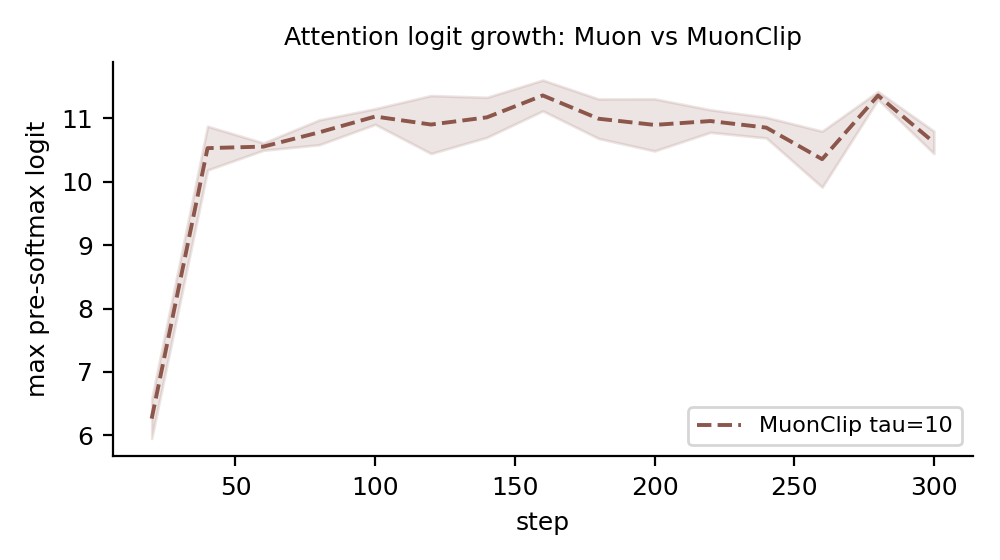
\includegraphics[width=0.72\textwidth]{../figures/logit_growth.pdf}
\caption{Max pre-softmax attention logit per step on TinyShakespeare. Without clipping (red), logits grow from 2 at initialization to 47 by step 200. With MuonClip $\tau{=}10$ (brown), logits are bounded at the threshold from around step 30 onward. At this model size the unconstrained growth causes no instability; at trillion-parameter scale the same growth reaches 1000+, at which point softmax saturates and loss spikes follow.}
\label{fig:logit}
\end{figure}

\Cref{fig:logit} shows the logit trajectories. Without clipping, max logits grow monotonically to 47 by step 200. With $\tau{=}10$, the clip fires from around step 30 and holds logits at the threshold. At 220k parameters this growth causes no instability; the clip removes signal the model was legitimately using, explaining the mild regularization in validation. At trillion-parameter scale the same growth reaches 1000+, softmax saturates, and the clip becomes a stability necessity rather than a regularizer. The experiment is a clean negative control: it confirms the mechanism works as described and that its benefit is specific to the scale where logit explosion is a genuine failure mode.

\subsection{Learning Rate Sensitivity}

\begin{figure}[t]
\centering
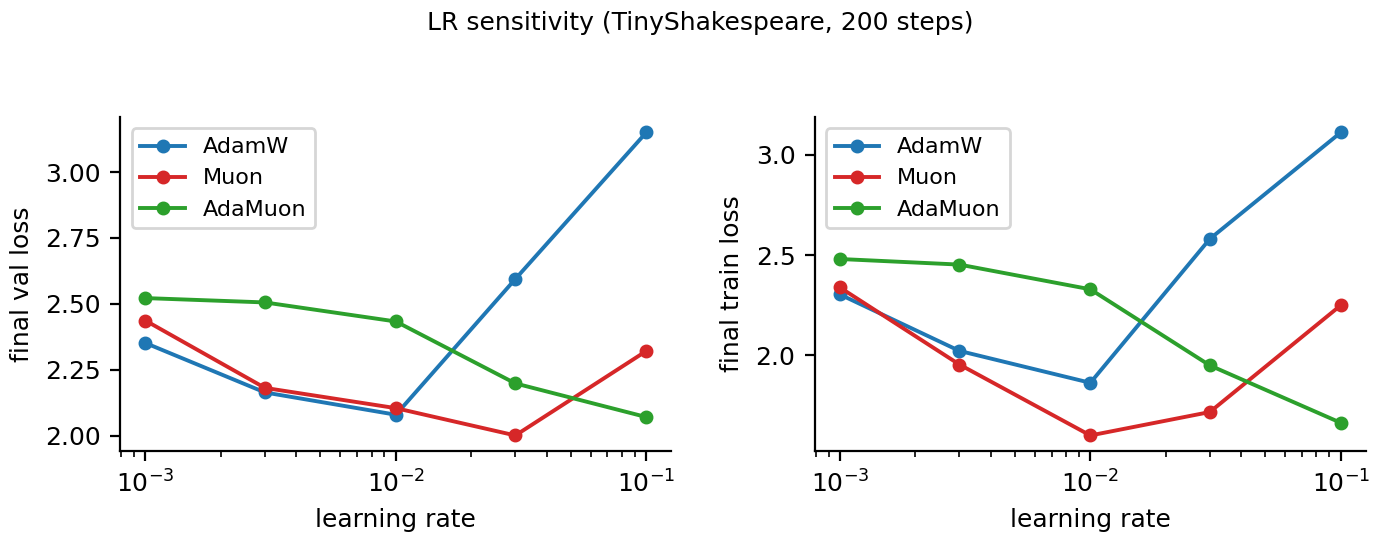
\includegraphics[width=0.9\textwidth]{../figures/lr_sweep.pdf}
\caption{LR sensitivity on TinyShakespeare (200 steps). Five learning rates are swept: $\{10^{-3},3{\times}10^{-3},10^{-2},3{\times}10^{-2},10^{-1}\}$. AdamW diverges at $\eta{=}10^{-1}$; Muon degrades gracefully across the full range.}
\label{fig:lr}
\end{figure}

The informal claim that Muon is more LR-sensitive than AdamW is wrong, at least for this task. \Cref{fig:lr} shows AdamW diverging at $\eta{=}10^{-1}$ (val loss 3.2 vs 2.1 at its best LR). Muon at $\eta{=}10^{-1}$ reaches val loss 2.3, a graceful degradation rather than divergence. The orthogonalized update has bounded operator norm by construction: the maximum singular value of each step is exactly 1 before scaling by $\eta$. This means the step size controls magnitude but not stability. AdamW has no such bound; at large LR the per-coordinate scaling can amplify gradient noise catastrophically in a single step.

The practical implication: AdamW baselines in optimizer comparisons need to include large learning rates in any tuning sweep, or the comparison understates how good AdamW can be. At the same time, Muon's robustness means that reported Muon numbers are less sensitive to the quality of hyperparameter search, which cuts the other way for fairness comparisons.

\subsection{Newton-Schulz Iteration Count}

\begin{figure}[t]
\centering
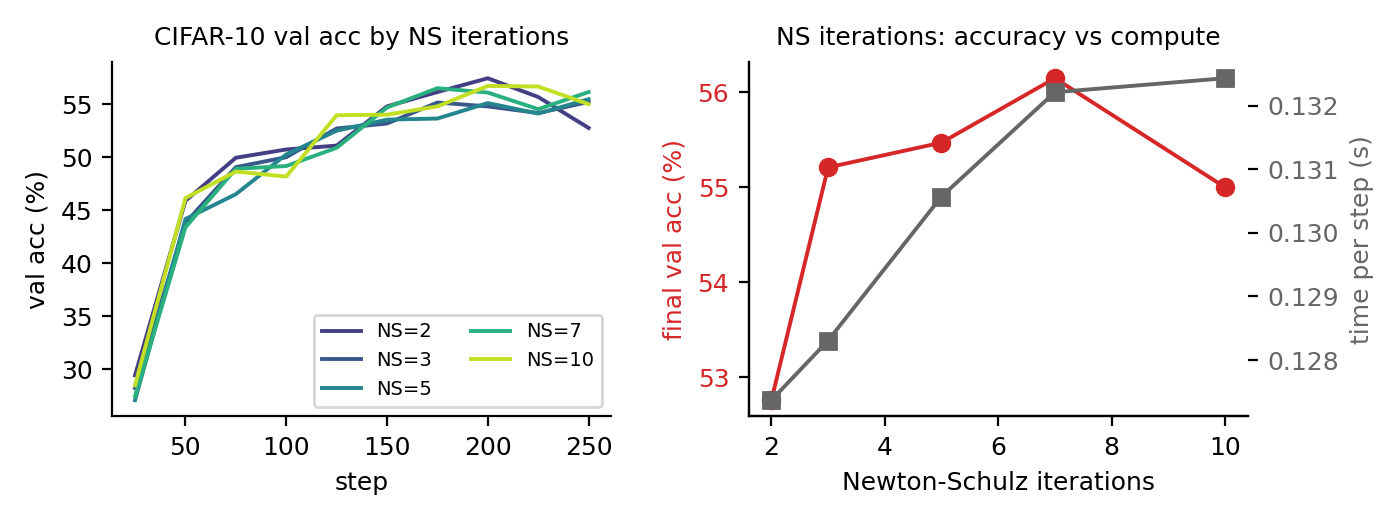
\includegraphics[width=0.9\textwidth]{../figures/ns_sweep.pdf}
\caption{NS iteration count $N\in\{2,3,5,7,10\}$ on CIFAR-10 (250 steps). Accuracy plateaus from $N{=}3$ onward. Per-step time grows linearly.}
\label{fig:ns}
\end{figure}

Validation accuracy for $N\in\{2,3,5,7,10\}$ is 53\%, 55\%, 55\%, 56\%, 55\%. The plateau from $N{=}3$ onward matches the mathematical expectation: the quintic polynomial is designed to converge quickly, and for weight matrices with moderate condition numbers (which small models tend to have) five iterations is more than enough. Per-step time grows linearly at roughly 0.5 ms per iteration, so $N{=}10$ costs 3.1\% more than $N{=}5$ with no benefit here. At larger scale, where weight matrices can have wider singular value distributions and smaller singular values take longer to reach 1, a higher $N$ might pay off.


\section{Discussion}
\label{sec:discussion}
\enlargethispage{2\baselineskip}

The experiments confirm that Muon's per-step advantage over AdamW is real at small scale, the variants are inconsistent, and MuonClip's benefit is scale-dependent in exactly the way the mechanism predicts.

\paragraph{The theory-practice gap is the main open problem.}
Shen et al.'s $\mathcal{O}(T^{-1/4})$ result proves Muon converges. It says nothing about why it converges faster than AdamW in practice. The right proof would exploit something about the geometry of the loss landscape that Muon's bounded-operator-norm update takes advantage of. The anisotropic Hessian measurements of \citet{dong2025quantifying} point toward a concrete direction: rates that depend on the spectral-vs-Frobenius gap of the loss landscape, where Muon's bounded operator norm would pay off proportionally.

\paragraph{Variant evaluation and the QK-Clip gap.}
AdaMuon beats Muon on one task and loses on another. Dion loses at small scale but would win in distributed training. MuonW is a marginal improvement on language modeling. MuonClip is essential at trillion-parameter scale and unnecessary below it. None of these rankings are stable across settings, and the literature lacks a benchmark that would let someone choose the right variant for a given scenario. The MuonClip case makes a deeper point: none of the 2025 convergence papers predicts that attention logit explosion would occur, because they treat the optimizer in isolation. The actual failure mode is a joint property of the optimizer and the attention mechanism. This is a gap in how the theory is set up, not just the tightness of the bounds.

Adam shipped with a flawed proof in 2014 and remained the default for a decade. Muon is on a similar trajectory. The field is at a point where the most valuable contributions are not more convergence upper bounds under slightly weaker assumptions, but better empirical methodology, scale-aware variant evaluation, and theory that treats the optimizer and model architecture as a coupled system. The MuonClip result makes this last point hard to ignore.

\clearpage
\bibliography{refs}
\end{document}
